%! Author = Luis
%! Date = 01.02.2024

% Beschreibung der Funktionen (z.B. mit Bildschirmfotos) sowie technischer Herausforderungen (Code-Schnippsel)


\chapter{Entwicklung}

\section{IpShare views}\label{sec:ip_share_views}
Die Tabelle \ref{tab: routes} zeigt alle implementierten Routen.
Zun{"a}chst die Einwicklung der IpShare views also der Routen, welche die Funktionalit{"a}t der Webseite ausmachen.

\begin{sidewaystable}[h]
    \centering
    \begin{tabular}{|l|l|l|l|l|}
        \hline
        \textbf{Blueprint} & \textbf{Route}                   & \textbf{Forms}                                                                                    & \textbf{Authentication} & \textbf{Methods}         \\
        \hline
        $ip\_share\_views$ & \tiny $/$                              &                                                                                                   &                         & HEAD, GET, OPTIONS       \\
        \hline
        $ip\_share\_views$ & \tiny $/now$                           & ShareNowForm                                                                                      &                         & HEAD, GET, POST, OPTIONS \\
        \hline
        $ip\_share\_views$ & \tiny $/impressum$                     &                                                                                                   &                         & HEAD, GET, OPTIONS       \\
        \hline
        $login\_views$     & \tiny $/register$                      & RegisterForm                                                                                      &                         & GET, OPTIONS, HEAD, POST \\
        \hline
        $login\_views$     & \tiny $/signin$                        & LoginForm                                                                                         &                         & GET, OPTIONS, HEAD, POST \\
        \hline
        $login\_views$     & \tiny $/signout$                       &                                                                                                   & login required          & GET, OPTIONS, HEAD       \\
        \hline
        $login\_views$     & \tiny $/me$                            & \parbox{5cm}{\vspace{1mm} ChangePseudonymForm \\ ChangePasswordForm \\ InvalidateTokensForm \\ SettingsForm \\ DeleteForm \vspace{1mm}} & fresh login required & GET, OPTIONS, HEAD, POST \\
        \hline
        $api\_views$       & \tiny $/v1/$                           &                                                                                                   &                         & HEAD, GET, OPTIONS       \\
        \hline
        $api\_views$       & \tiny $/v1/$                           &                                                                                                   &                         & PUT, OPTIONS             \\
        \hline
        $api\_views$       & \tiny $/v1/$                           &                                                                                                   &                         & DELETE, OPTIONS          \\
        \hline
        $api\_views$       & \tiny $/v1/token/<device\_name>$ &                                                                                                   &                         & HEAD, GET, OPTIONS       \\
        \hline
        $qr\_views$        & \tiny $/qr/<addr>$               &                                                                                                   &                         & HEAD, GET, OPTIONS       \\
        \hline
        & \tiny $/static/<filename>$       &                                                                                                   &                         &                          \\
        \hline
    \end{tabular}
    \caption{Routen}
    \label{tab: routes}
\end{sidewaystable}


\subsection{Hauptseite}\label{subsec:hauptseite}
Serverseitig ist die Hauptseite simple.
Der Server ermittelt lediglich die Ip-Adresse des Clients und rendert die $index.html$.
Daf{"u}r ist die Komplexit{"a}t clientseitig h{"o}her.
Das $index.js$ {"u}bernimmt die Kommunikation mit dem Socket, n{"a}her beschrieben im Abschnitt~\ref{sec:socket}, um die Address-Tabellen zu f{"u}llen.
Beim Klicken auf den Namen, den Token oder die Adresse werden diese entsprechend in die Zwischenablage kopiert.
Die Icons andern sich, wenn mit der Maus {"u}ber sie gehoverd wird.
Durch Klicken auf die Edit-Icons (Stift-Symbol) werden die Felder zur eingabe des Device-Namen und der Adresse sowie Token und QR-Code angezeigt.
QR-Code und Token werden hierbei in Abh{"a}ngigkeit der Adresse und Device-Namen vom Server bezogen.
Mehr dazu in den Abschnitten zu Token~\ref{subsec:token} und QR-Code~\ref{sec:qr}.

\subsection{Jetzt Teilen Route}\label{subsec:jetzt-teilen-roote}
{"U}ber die $/now$ Route k{"o}nnen User ihre Ip-Adresse sofort Teilen.
Ist der Client authentifiziert, wird die $share\_ip\_now()$ Funktion aus Abschnitt~\ref{subsec:jetzt-teilen-funktion} aufgerufen und auf die Hauptseite weitergeleitet.
Ist der Client nicht authentifiziert, wird $now.html$ mit dem $ShareNowForm$ gerendert.
Hier wird der Visitor nochmal gefragt, ob er sich der Risiken des ver{"o}ffentlichen bewusst ist.
Das verhindert auch das jemand eine Url untergejubelt bekommt, die dann unfreiwillig seine IP ver{"o}ffentlicht.
Ich will nicht ausschlie\ss en, das dies nicht trotzdem m{"o}glich ist, aber zumindest ist es nicht so einfach.

\subsection{Jetzt Teilen Funktion}\label{subsec:jetzt-teilen-funktion}
Die $share\_ip\_now()$ Funktion ist f{"u}r das Teilen der vom Server automatisch ermittelten Funktion zust{"a}ndig.
Der Server ermittelt die {"o}ffentliche Ip-Adresse des Clients wie in Listings~\ref{lst:views} gezeitigt anhand der environment Variablen.
Die grundlage f{"u}r den Programmcode ist hierf{"u}r von Tirtha Rahaman~\cite{getip}.
\lstinputlisting[firstline=19, firstnumber=19, lastline=22, caption=views.py, label={lst:views}]{../../app/views.py}
Wenn die Address bereits in der DB ist, wird sie nur aktualisiert ansonsten wird sie neu angelegt.
Je nachdem ob ein authentifizierter User oder ein Visitor teilt, wird der Device-Name anders ermittelt.
Bei einem User wird aus dem User-Agent-Header der Browser und das Betriebssystem ermittelt.
Bei mir w{"a}hre das z.B. ``Firefox Windows''.
F{"u}r den Visitor wird ein Globaler Z{"a}hler verwendet, der einfach f{"u}r jede Address um eins hochz{"a}hlt.
Zuletzt wird noch ein Socket Event emittiert, um alle Client Tabellen zu aktualisieren.

\subsection{Impressum}\label{subsec:impressum}
Die Impressum Route rendert lediglich das Impressum aus $impressum.html$.


\section{Socket}\label{sec:socket}
Um die Tabellen der User aktuell zu halten ohne das dieser refreshen muss verwende ich Flask-SocketIO~\cite{socket}.
Zu empfehlen ist hier auch das Video vom Entwickler selbst: \url{https://youtu.be/OZ1yQTbtf5E?si=2_tiaAlKpT-p9HCP}
Ich habe mich hier entgegen seinem anraten f{"u}r eine Read-Only-Session entschieden.
Denn in meinem Fall m{"o}chte ich die Session nicht {"u}ber das Socket {"a}ndern.
\begin{samepage}
    Es sind f{"u}nf Events implementiert auf die der Server reagiert:
    \begin{itemize}
        \setlength\itemsep{-0.4em}
        \item connect - beginnt die Kommunikation nach dem Verbindungsaufbau.
        \item disconnect - beendet die Kommunikation nach dem Verbindungsabbau.
        \item now - Teilen der Ip Adresse mittels $share\_ip\_now()$.
        \item save - speichert bzw. aktualisiert eine Adresse.
        \item delete - l{"o}scht eine Adresse.
    \end{itemize}
\end{samepage}

\begin{samepage}
    F{"u}r den Client sind drei Events implementiert:
    \begin{itemize}
        \setlength\itemsep{-0.4em}
        \item user authenticated - setzt die $user\_authenticated$ Variable des Client.
        \item user table - {"u}bermittelt die User Adressdaten f{"u}r die User-Table.
        \item public table - {"u}bermittelt die {"o}ffentlichen Adressdaten f{"u}r die Public-Table.
    \end{itemize}
\end{samepage}

Die $connect$ Funktion sendet die Tabellendaten und emittiert das $user authenticated$ Event.
Au\ss erdem betritt der Client den $room$ des Users.
So kann ein User mehrere Tabs {"o}ffnen, die sich gegenseitig aktualisieren.
Beim Verlassen wird die $disconnect$ Funktion aufgerufen.
Ein authentifizierter Client verl{"a}sst hier den User room.
Ein Visitor l{"o}scht seine Adresse aus der Datenbank.
Wenn ein Visitor seinen Tab schlie\ss t, wird seine Adresse also aus der Datenbank entfernt und somit nicht mehr geteilt.
Die $save$ und $delete$ Events sind, denke ich selbst erkl{"a}rend.
Sie Speichern, Aktualisieren oder L{"o}schen die {"u}bermittelte Adresse.
Die $user table$ und $public table$ Events {"u}bermitteln die Daten im JSON Format.
\begin{samepage}
    Das sieht dann z.B. so aus:
    \begin{lstlisting}
[{"device_name": "Firefox Windows", "address": "127.0.0.1", "last_updated": "5 days ago"},
{"device_name": "Broadcast", "address": "255.255.255.255", "last_updated": "5 days ago"}]
    \end{lstlisting}
\end{samepage}


\section{Login und User Management}\label{sec:login_views}
Das User Management System verwendet Flask-Login und Flask-Bcrypt als Grundlage.
{"U}ber die $/register$ Route kann sich ein User einen Account mit Username und Passwort anlegen.
Er kann au\ss erdem w{"a}hlen ob er eine remember-me-Cookie m{"o}chte.
Sollte er sich dazu entscheiden wird er automatisch eingeloggt, wenn er die Webseite {"o}ffnet.
Ansonsten kann er sich entsprechend {"u}ber die $/signin$ Route einloggen.
{"U}ber $/signout$ kann sich der User wider abmelden.
Beim registrieren und einloggen k{"o}nnen Nachrichten angezeigt werden.
Zum Beispiel das ein Benutzername schon in Verwendung ist oder das Passwort falsch eingegeben wurde.
Auch noch wichtig ist die $load\_user$ Funktion, welche den User aus der Datenbank abfr{"a}gt.
Als kleines extra kann mit der $redirect\_next$ Funktion ein User an eine bestimmte Adresse weitergeleitet werden.
Das ist praktisch wenn ein User z.B. auf die $/me$ Route m{"o}chte aber nicht authentifiziert ist.
Dann wird er zu $/signin$ weitergeleitet und nach dem login wider zur{"u}ck zu $/me$.
Wo wir schon dabei sind die $/me$ Route erlaubt es dem User sein Username/Pseudonym anzupassen,
sein Passwort zu {"a}ndern, seine Token zu invalidieren und seine remember-me-Cookie Einstellungen zu {"a}ndern.
Er kann auch seinen Account l{"o}schen.
Diese $/me$ Route ist durch klicken auf den Nutzernamen rechts oben erreichbar.

\section{API}\label{sec:api_views}
Die API ist recht simple gehalten.
Adressen k{"o}nnen abgerufen, hochgeladen und gel{"o}scht werden.
Der Token {"u}bernimmt hier bei nicht nur die Authentifizierung sondern gib auch gleich an um welche Adresse von welchem User es sich handelt.
Das Abrufen kann dann z.B. in Python mit dem requests Paket wie folgt durchgef{"u}hrt werden:

\vspace{3mm}
\begin{lstlisting}
    import requests
    headers = {"Authorization": f"Bearer APITOKEN"}
    print(requests.get("http://127.0.0.1:5000/v1/", headers=headers).text)
\end{lstlisting}
\vspace{3mm}

Hochladen oder Aktualisieren funktioniert wie folgt:
\vspace{3mm}
\begin{lstlisting}
    import requests
    headers = {"Authorization": f"Bearer APITOKEN"}
    data = "2.3.4.5"
    requests.put("http://127.0.0.1:5000/v1/", data=data, headers=headers)
\end{lstlisting}
\vspace{3mm}

Auch das L{"o}schen ist leicht:
\vspace{3mm}
\begin{lstlisting}
    import requests
    headers = {"Authorization": f"Bearer APITOKEN"}
    requests.delete("http://127.0.0.1:5000/v1", headers=headers)
\end{lstlisting}
\vspace{3mm}

\subsection{Token}\label{subsec:token}
Die API erm{"o}glicht es auch den Token f{"u}r einen Device-Name auszustellen.
Diese Funktion ist aber nicht direkt f{"u}r den User gedacht.
Sie wird vom $index.json$ verwendet um den Token in der EDIT-Ansicht zum Kopieren zur verf{"u}gung zu stellen.
Der User sollte also erst manuel eine Adresse anlegen um den Token zu erhalten.

Um die Token zu invalidieren ben{"o}tigt jeder user einen alternative\_id die sich {"a}ndern kann.
Die Token werden auf die alternative\_id ausgestellt.
Um die Token zu invalidieren wird die alternative\_id ge{"a}ndert.
Alle Token sind dann f{"u}r einen nicht existenten User und somit ung{"u}ltig.

Bei den Token handelt es sich um JSON Web Tokens (JWT) welche mit der PyJWT Library~\cite{jwt} erstellt werden.
Wie Abbildung~\ref{fig: jwt} zeigt beinhaltet der Token die alternative\_id des User und den Device-Name.
Diese Decodierung kann auf \url{https://jwt.io/#debugger-io} durchgef{"u}hrt werden.
Hier ist auch noch etwas Optimierungspotential was die Payload gr{"o}\ss e Betrifft.
Das Vorgehen beim einbinden des Token in den Header ist von cassiomolin\cite{cassiomolin}.

\begin{figure}[h]
    \centering
    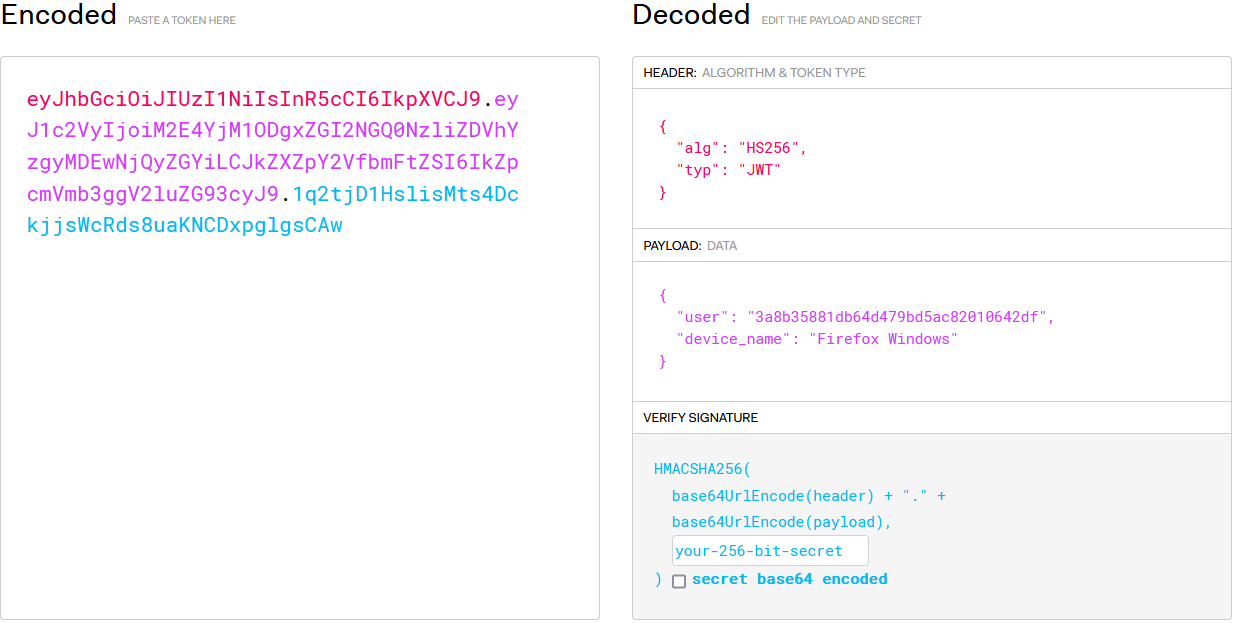
\includegraphics[width=\textwidth]{jwt}
    \caption{Beispiel jwt}
    \label{fig: jwt}
\end{figure}

\section{QR-Code}\label{sec:qr}
Die QR-Codes werden mit der qrcode Bibliothek erstellt und im Anschluss mit OpenCV nachbearbeitet.
Zum versenden m{"u}ssen sie noch ins PNG Rastergrafikformat konvertiert werden.
Dazu wird die Python Imaging Library (PIL) names Pillow verwendet.
Um die Datei nicht im System speichern zu m{"u}ssen wird in einen binary stream geschrieben.
Dieser wird von der io Library {"u}ber BytesIO durch einem in-memory byte buffer zur Verf{"u}gung gestellt.
Mehr dazu unter \url{https://docs.python.org/3/library/io.html#io.BytesIO}.
Noch zu Erw{"a}hnen ist das vor dem Sender der ```Lesekopf'' noch mit $fp.seek(0)$ an den Anfang gesetzt werden muss.

\subsection{encodeURI}\label{subsec:encodeuri}
Eine Schwierigkeit war hier die Address in der Url an die Api mitzugeben.
Das man eine URL nicht einfach in eine URL schreiben kann ist irgendwo auch einleuchtend.
Dieses Problem hat auch die Token API aus dem vorherigen Abschnitt.
Dort ist es nur vielleicht nicht sofort erkenntlich.
Aber auch ein Device-Name kann in einer URL unerlaubte zeichen wie ;/?:@\&=+\$,\# enthalten.
Die Zeichen m{"u}ssen also escaped werden.
Auf JavaScript seite kommt hier $encodeURI()$\cite{encodeURI} zum einsatz.
W{"a}hrend in Python die $unquote\_plus()$\cite{unquoteplus} Funktion aus der urllib verwendet wird.


\section{Cookies}\label{sec:cookies}
Als Visitor soll die Seite ohne Cookies verwendet werden k{"o}nnen.
Dann muss der Visitor keinen nervigen Cookie Banner wegklicken.
Als eingeloggter User wird ein Session-Cookie ben{"o}tigt.
Optional kann ein User auch noch einen Remember-Me-Cookie bekommen.
Um die Cookies von Flask f{"u}r Visitors zu unterbinden wird ein CustomSessionInterface ben{"o}tigt.
Dieses {"u}berschreibt die $should\_set\_cookie()$ Funktion so das kein Cookie gesendet wird wenn der user nicht authentifiziert ist.
Leider bringt das einige Schwierigkeiten mit sich.
Die (Cross-Site-Request-Forgery) CSRF Tokens f{"u}r die Flask-Forms ben{"o}tigen eigentlich Sessions.
Ich musste daher extra ein SessionLessCSRF Token verwenden der {"u}ber die Ip-Adresse funktioniert.
Dieser ist allerdings nicht sehr sicher.
Daher kommt der spezial Token nur f{"u}r die register, signin und share\_now Forms zum Einsatz.
Um diese Forms zu verwenden muss der User ohnehin nicht eingeloggt sein.
Ein Angreifer kann auch so einen Account registrieren oder eine Adresse teilen.

Gelegentlich funktionierte in meinen Tests der Logout nicht richtig.
Dann musste ich die Cookies manuel l{"o}schen.
Mir ist nicht bekannt woran das liegt, da ich Schwierigkeiten habe den Fehler zu Reproduzieren.
Es hat aber m{"o}glicherweise etwas mit dem CustomSessionInterface zutun.

\section{APScheduler}\label{sec:ap_scheduler}
Flask f{"u}hrt normaler weise nur Funktionen aus, um auf eine Anfrage zu reagieren.
Um alte Visitor Adressen nach einer Zeit zu entfernen wird daher der flask\_apscheduler ben{"o}tigt.
Mit ihm l{"a}sst sich die $clear\_old\_visitor\_addrs()$ Funktion jede minute aufrufen.
Diese kontrolliert dann ob eine Visitor Adresse {"a}lter als 42 Minuten ist und l{"o}scht diese gegebenenfalls.

\section{Scramble Effect}\label{sec:scramble-effect}
Um die Seite etwas spannender zu gestalten zeige ich einen Scramble Effect beim hovern {"u}ber Links und Buttons.
Der Effect ist in $scramble.js$ implementiert und wurde durch \href{https://youtu.be/W5oawMJaXbU}{HYPERPLEXED} inspiriert.
Welcher sich wiederum von \href{https://kprverse.com}{KPR} inspirieren hat lassen.
Der \href{https://codepen.io/Hyperplexed/pen/rNrJgrd'}{codepen} zum vergleich.
Im Prinzip werden die Zeichen durch Zuf{"a}llige Zeichen ersetzt und dann langsam die Tats{"a}chlichen Zeichen wider angezeigt.
Die Zeichen k{"o}nnen durch Zahlen, Buchstaben oder Punkte ersetzt werden.
Die $now.js$ und $register.js$ implementieren eine {"A}hnliche funktion um einen Typewriter Effect f{"u}r die Informationen zu erzeugen.

\section{Checkbox}\label{sec:checkbox}
\lstset{basicstyle=\selectfont\ttfamily, language=CSS}

Da die Standard Checkboxen optisch nicht zur Webseite passten habe ich welche mit css erstellt.
Eine Schwierigkeit hierbei war das css nicht zwischen absoluter und relativer Positionierung animieren kann.
Im unchecked Zustand Abbildung~\ref{fig: unchecked} sollte die box relativ zum Text positioniert werden.
Im checked Zustand Abbildung~\ref{fig: checked} sollte die box absolut um den Text positioniert werden.
Um ein Saubere Animation zu erhalten habe ich mich f{"u}r absolute positionierung entschieden.
Die Box wird im unchecked Zustand mithilfe einer variablen \lstinline$--chars$ positioniert.
Diese Variable muss f{"u}r jede checkbox im html auf die Anzahl der Zeichen gesetzt werden.
Im css wird die Positionierung der linken Kannte im unchecked Zustand dann mit \lstinline$left: calc(11.7rem - var(--chars) / 2);$ berechnet.
Das Html f{"u}r eine Checkbox ist dann entsprechend so:

\lstset{basicstyle=\fontsize{7}{8}\selectfont\ttfamily, language=HTML5}
\vspace{3mm}
\begin{lstlisting}
    <div class="checkbox-container" style="--chars: 10ch;">
        {{ settings_form.remember }}
        <label for="remember">REMEMBER ME</label>
    </div>
\end{lstlisting}
\vspace{3mm}

\begin{minipage}[h]{0.425\textwidth}
    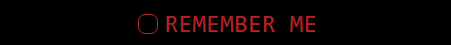
\includegraphics[width=\textwidth]{unchecked}
    \captionof{figure}{unchecked Checkbox}
    \label{fig: unchecked}
\end{minipage}
\hspace{0.05\textwidth}
\begin{minipage}[h]{0.425\textwidth}
    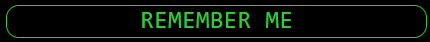
\includegraphics[width=\textwidth]{checked}
    \captionof{figure}{checked Checkbox}
    \label{fig: checked}
\end{minipage}


\section{Limiter}\label{sec:limiter}
Um sich gegen DOS-Attacken zu wehren kann mit dem Flask-limiter f{"u}r jede Route ein limit gesetzt werden.
So k{"o}nnen f{"u}r rechenintensivere Funktionen wie z.B. die Qr-Code erzeugung strengere Grenzen eingestellt werden.
Die Limits sind {"u}ber die Dekoratoren $@limiter.limit()$ vor den Routen festgelegt.
Diese Funktionalit{"a}t habe ich auch leicht zweckentfremdet um die Login Versuche zu limitieren.

\section{Tests}\label{sec:tests}
\lstset{basicstyle=\selectfont\ttfamily}

Auch an den Tests wollte ich mich zumindest kurz versuchen.
Ab besten sind dabei die Tests f{"u}r die API.
Der Test f{"u}r die $/now$ Route in $test\_views$ ist leider nicht mehr aktuell.
Die Unit-Tests sind nicht ganz leicht, da in den Funktionen auf die Datenbank zugegriffen wird.
Auch die Authentifizierung muss ber{"u}cksichtigt werden.
Ob und wie sich das JavaScript automatisiert testen l{"a}sst ist auch noch unklar.
Recht hilfreich empfinde ich die coverage Reports die in der Konsole mit \lstinline$python -m pytest --cov-report=html --cov$ erstellt werden k{"o}nnen.
